\documentclass{beamer}
\usetheme{Warsaw}

\usepackage{amsfonts} % math symobls
\usepackage{amsthm}
\usepackage[utf8]{inputenc}
\usepackage{polski}
\usepackage{graphics}
\usepackage{verbatim}

\newcommand{\emp}[1]{\textcolor{blue}{\textit{#1}}}
\newcommand{\red}[1]{\textcolor{red}{#1}}

\title{Rozpoznawanie chorób skóry}
\author{Michał Karpiński}
\date{24 stycznia, 2013}

\begin{document}

\begin{frame}[plain]
  \titlepage
\end{frame}

\begin{frame}{Choroby skóry}

\begin{columns}
\begin{column}{0.5\textwidth}
\begin{center}
  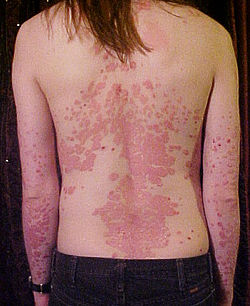
\includegraphics[scale=0.5]{img/psoriasis.jpg}

  Łuszczyca
\end{center}
\end{column}
\begin{column}{0.5\textwidth}
\begin{center}
  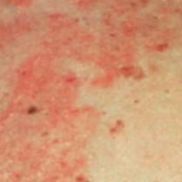
\includegraphics[scale=0.5]{img/seboreic_dermatitis.jpeg}  

  Łojotokowe zapalenie skóry
\end{center}
\end{column}
\end{columns}
\end{frame}

\begin{frame}{Choroby skóry}

\begin{columns}
\begin{column}{0.5\textwidth}
\begin{center}
  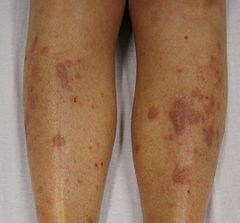
\includegraphics[scale=1.5]{img/lichen_planus.jpg}

  Liszaj płaski
\end{center}
\end{column}
\begin{column}{0.5\textwidth}
\begin{center}
  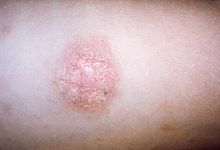
\includegraphics[scale=1.5]{img/pityriasis_rosea.jpg}  

  Łupież różowy Giberta
\end{center}
\end{column}
\end{columns}
\end{frame}

\begin{frame}{Choroby skóry}

\begin{columns}
\begin{column}{0.5\textwidth}
\begin{center}
  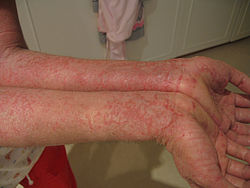
\includegraphics[scale=0.7]{img/chronic_dermatitis.jpg}

  Atopowe zapalenie skóry
\end{center}
\end{column}
\begin{column}{0.5\textwidth}
\begin{center}
  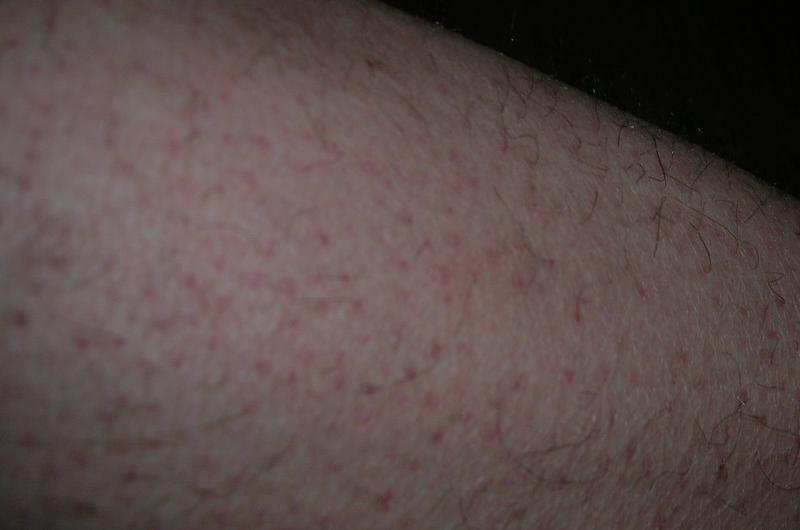
\includegraphics[scale=0.2]{img/pityriasis_rubra_pilaris.jpg}  

  Rogowacenie przymieszkowe czerwone
\end{center}
\end{column}
\end{columns}
\end{frame}

\begin{frame}{Dane}
\begin{block}{Źródło}
{\em http://archive.ics.uci.edu/ml/datasets/Dermatology}
\end{block}

\begin{itemize}
\item Liczba próbek: 366
\item Liczba cech: 34
\item Liczba klas: 6
\end{itemize}

\end{frame}

\begin{frame}{Dane - liczba osobników w danej klasie}

\begin{center}
  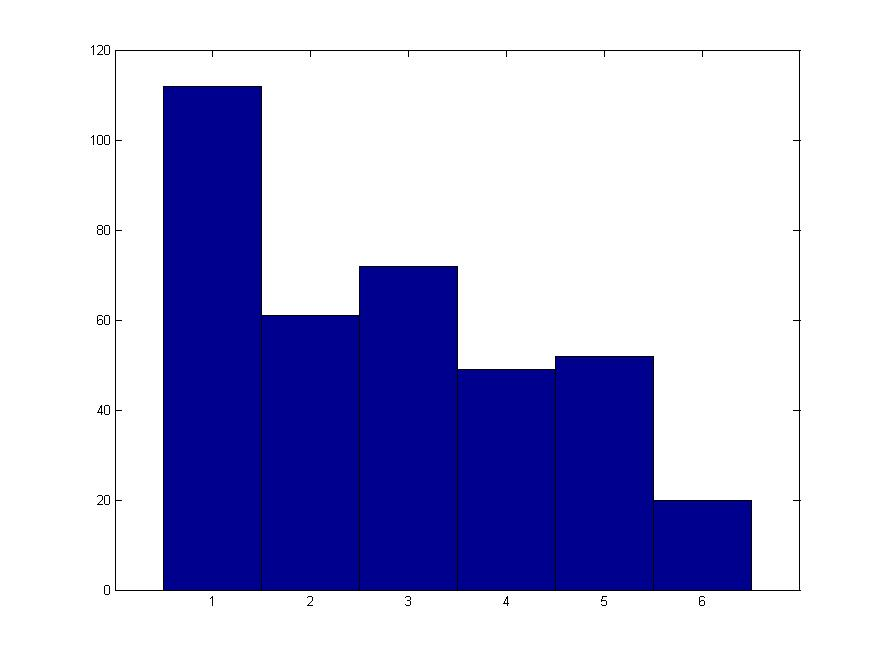
\includegraphics[scale=0.35]{img/class_hist.jpg}  
\end{center}

\end{frame}

\begin{frame}{Dane - cechy kliniczne}
  \begin{itemize}
    \item zaczerwienienie
    \item skala zmian
    \item swędzenie
    \item kształt
    \item miejsce występowania
    \item wiek
    \item występowanie choroby w rodzinie
  \end{itemize}
\end{frame}

\begin{frame}{Dane - cechy histopatologiczne}
\begin{itemize}
\item PNL infiltrate
\item exocytosis
\item acanthosis
\item hyperkeratosis
\item parakeratosis
\item clubbing of the rete ridges
\item elongation of the rete ridges
\item thinning of the suprapapillary epidermis
\item spongiform pustule
\item munro microabcess
\item focal hypergranulosis
\item spongiosis
\item saw-tooth appearance of retes
\item follicular horn plug
\item perifollicular parakeratosis
\item band-like infiltrate
\end{itemize}
\end{frame}

\begin{frame}{Dane - dziedzina cech}
Wartości wszystkich cech zmierzone zostały w czterostopniowej skali \{0,1,2,3\}.

\vspace{0.5cm}

Wyjątki:
\begin{itemize}
\item występowanie choroby w rodzinie - \{0,3\}
\item wiek - liczba naturalna
\end{itemize}

\end{frame}

\begin{frame}{Standaryzacja wieku}

\begin{center}
  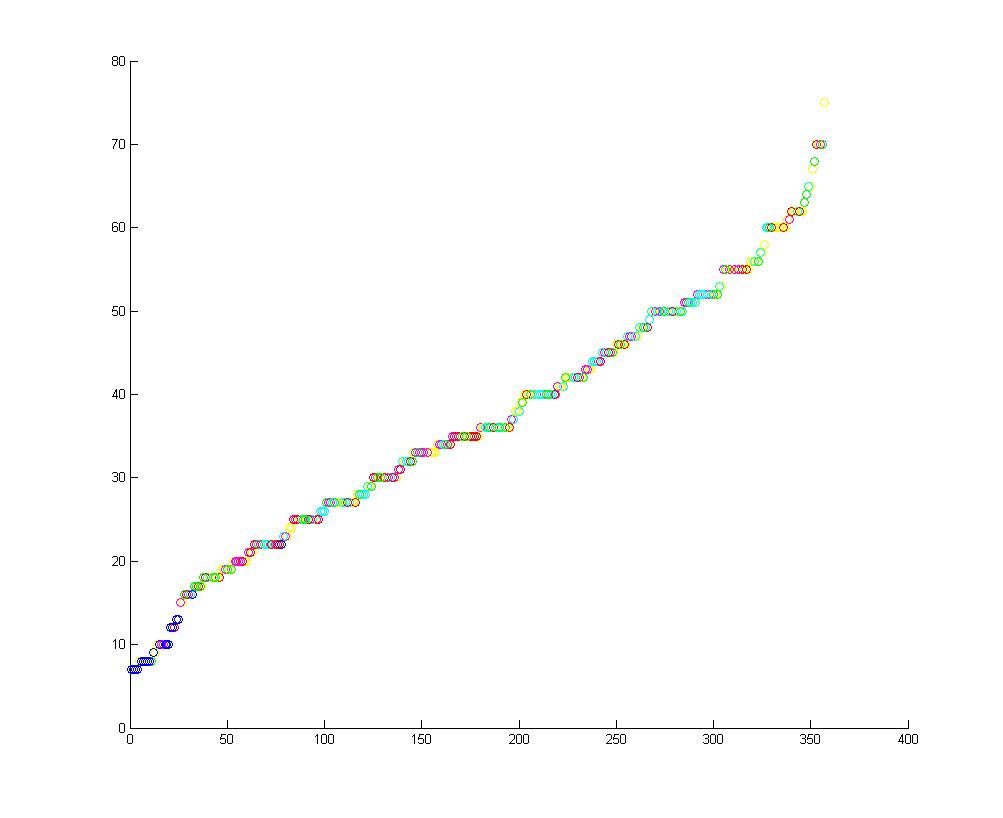
\includegraphics[scale=0.3]{img/age_scatter.jpg}  
\end{center}

\end{frame}

\begin{frame}{Standaryzacja wieku}
\begin{center}

Standaryzujemy wiek zgodnie z poniższą tabelą:

\vspace{0.5cm}

{\LARGE 
\begin{tabular}{ | c | c | }
  \hline
  $(0,17\rangle$ & 0 \\
  $(18,40\rangle$ & 1 \\
  $(41,55\rangle$ & 2 \\
  $(56,\infty)$ & 3 \\
  \hline
\end{tabular}
}
\end{center}
\end{frame}

\begin{frame}{Analiza danych}

\begin{center}
  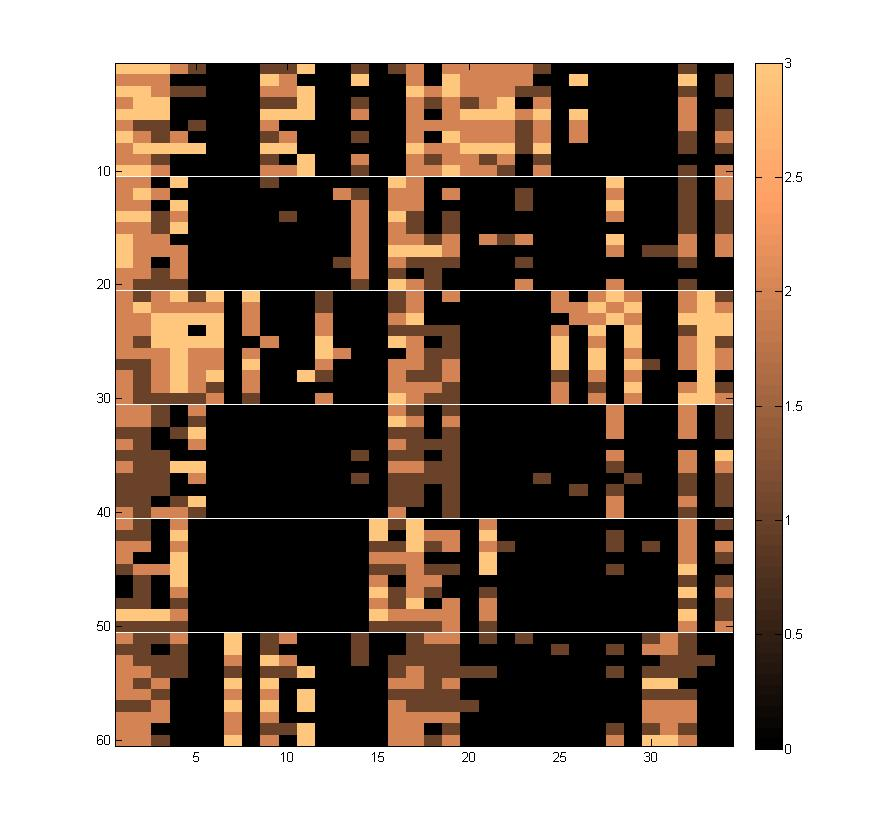
\includegraphics[scale=0.3]{img/data_imagesc.jpg}  
\end{center}

\end{frame}

\begin{frame}{Sieć neuronowa - MLP}
\begin{itemize}
\item pakiet netlab (mlptrain, mlpfwd)
\item sieć dwuwarstwowa
\item jedna warstwa ukryta z osmioma neuronami
\item wejście długości 34
\item wyjście długości 6
\item liniowa funkcja aktywacji
\item 100 iteracji 
\end{itemize}
\end{frame}

\begin{frame}{5-fold cross-validation}
 Średni błąd: 0.0223
\vspace{0.5cm}

\begin{center}
{\LARGE 
\begin{tabular}{ | c | c | c | c | c | c |}
\hline
   22.4  &       0  &       0  &       0 &        0  &       0 \\ \hline
         0  & 10.4  &       0  &  1.8 &        0  &       0 \\ \hline
         0  &       0  & 14.4  &       0 &        0  &       0 \\ \hline
         0  &  0.8  &       0  &  9.0 &        0  &       0 \\ \hline
         0  &       0  &       0  &       0 &  10.0  &       0 \\ \hline
         0  &       0  &       0  &       0 &        0  &  4.0 \\ \hline
\end{tabular}
}
\end{center}
\end{frame}

\begin{frame}{5-fold cross-validation}
\begin{center}
  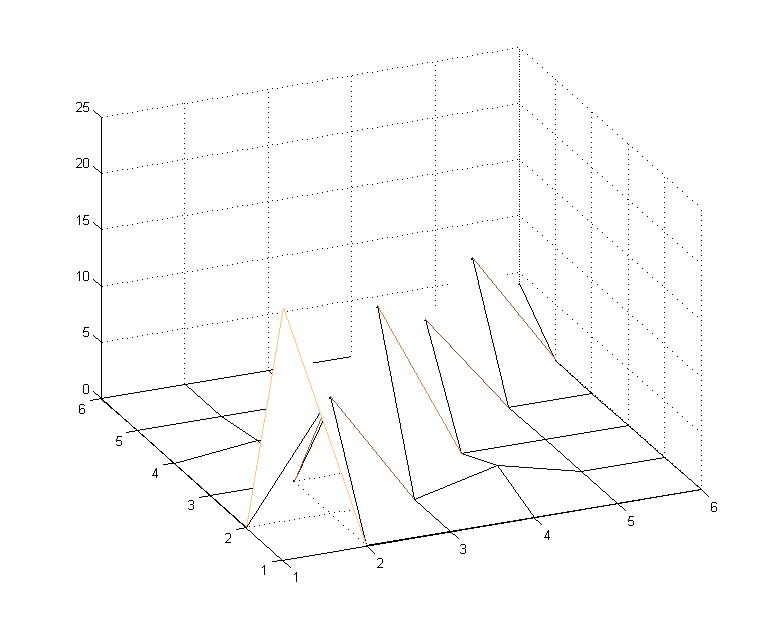
\includegraphics[scale=0.35]{img/mp_mesh.jpg}  
\end{center}
\end{frame}

\begin{frame}{Drzewo decyzyjne}

 {\bf Weka} - program wspierający obliczenia i wizualizacje systemów uczących się.

\vspace{0.5cm}

\begin{block}{Źródło}
http://www.cs.waikato.ac.nz/ml/weka/
\end{block}
\end{frame}

\begin{frame}{Pierwsza przymiarka}
\begin{center}
  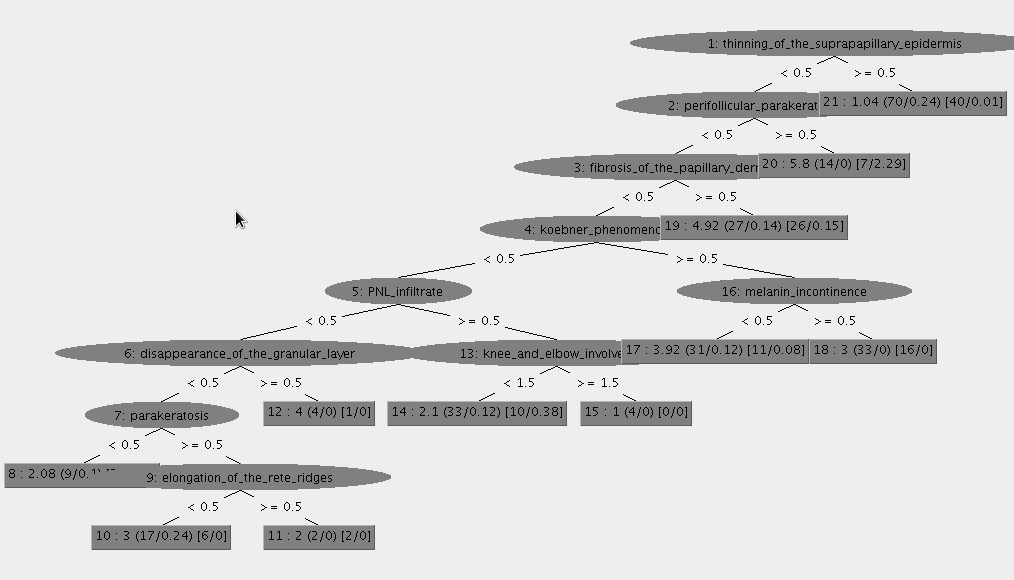
\includegraphics[scale=0.30]{img/decision_tree1.png}  
\end{center}
\end{frame}

\begin{frame}{Druga przymiarka}
\begin{center}
  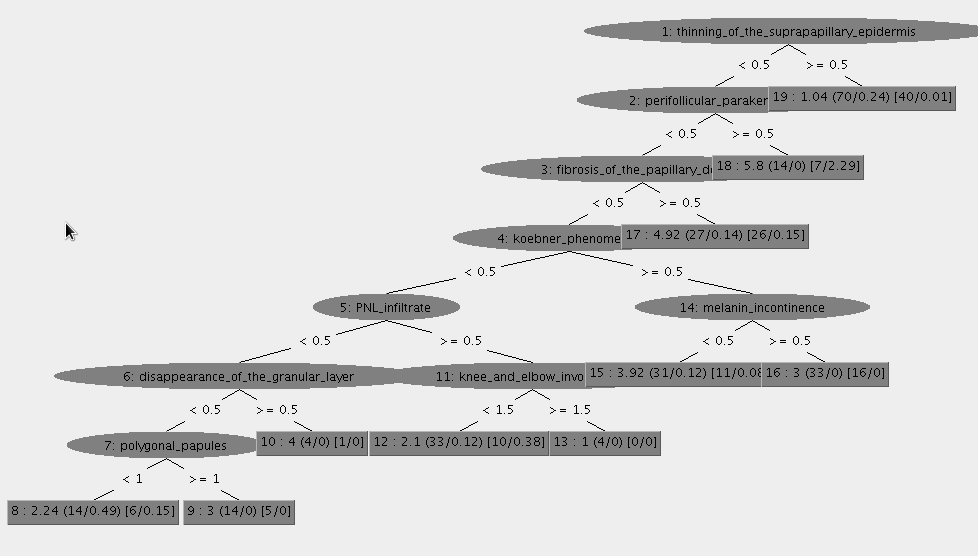
\includegraphics[scale=0.30]{img/decision_tree2.png}  
\end{center}
\end{frame}

\begin{frame}{Błąd klasyfikacji}
\begin{itemize}
\item przed usunięciem wybranych cech: 0.1851
\item po usunięciu wybranych cech: 0.2049
\end{itemize}
\end{frame}


\begin{frame}{5-fold cross-validation - runda druga}
 Średni błąd: 0.0733
\vspace{0.5cm}

\begin{center}
{\LARGE 
\begin{tabular}{ | c | c | c | c | c | c |}
\hline
   22.4  &       0  &       0  &       0  &       0  &       0 \\ \hline
    0.2  & 11.0  &       0  &  0.4  &  0.6  &       0 \\ \hline
         0  &       0  & 14.2  &       0  &  0.2  &       0 \\ \hline
         0  &  1.0  &  0.2  &  8.6  &       0  &       0 \\ \hline
         0  &       0  &       0  &       0  & 10.4  &       0 \\ \hline
         0  &       0  &       0  &       0  &       0  &  4.0 \\ \hline
\end{tabular}
}
\end{center}
\end{frame}


\end{document}
